% Created by tikzDevice version 0.12.6 on 2025-04-07 10:13:20
% !TEX encoding = UTF-8 Unicode
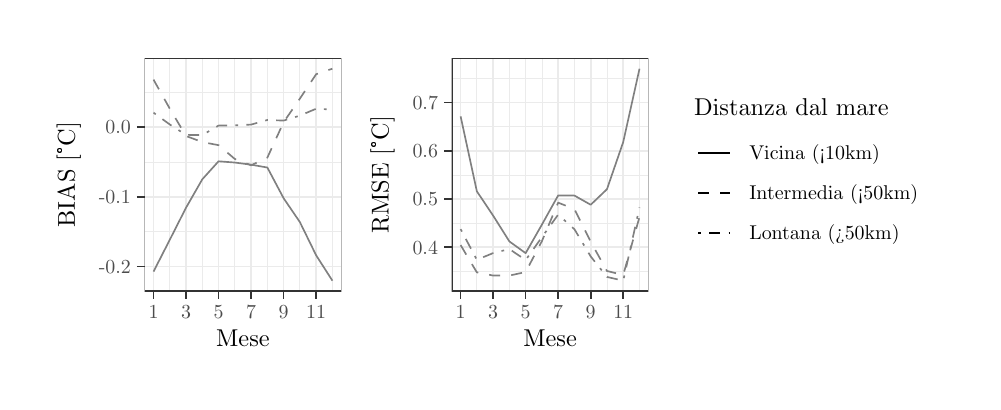
\begin{tikzpicture}[x=1pt,y=1pt]
\definecolor{fillColor}{RGB}{255,255,255}
\path[use as bounding box,fill=fillColor] (0,0) rectangle (341.43,128.04);
\begin{scope}
\path[clip] (  0.00,  0.00) rectangle (341.43,128.04);
\definecolor{drawColor}{RGB}{255,255,255}

\path[draw=drawColor,line width= 0.6pt,line join=round,line cap=round,fill=fillColor] (  0.00,  0.00) rectangle (341.43,128.04);
\end{scope}
\begin{scope}
\path[clip] (  5.50,  5.50) rectangle (118.85,122.54);
\definecolor{drawColor}{RGB}{255,255,255}
\definecolor{fillColor}{RGB}{255,255,255}

\path[draw=drawColor,line width= 0.6pt,line join=round,line cap=round,fill=fillColor] (  5.50,  5.50) rectangle (118.85,122.54);
\end{scope}
\begin{scope}
\path[clip] (118.85,  5.50) rectangle (335.93,122.54);
\definecolor{drawColor}{RGB}{255,255,255}
\definecolor{fillColor}{RGB}{255,255,255}

\path[draw=drawColor,line width= 0.6pt,line join=round,line cap=round,fill=fillColor] (118.85,  5.50) rectangle (335.93,122.54);
\end{scope}
\begin{scope}
\path[clip] ( 42.24, 32.79) rectangle (113.35,117.04);
\definecolor{fillColor}{RGB}{255,255,255}

\path[fill=fillColor] ( 42.24, 32.79) rectangle (113.35,117.04);
\definecolor{drawColor}{gray}{0.92}

\path[draw=drawColor,line width= 0.3pt,line join=round] ( 42.24, 54.36) --
	(113.35, 54.36);

\path[draw=drawColor,line width= 0.3pt,line join=round] ( 42.24, 79.52) --
	(113.35, 79.52);

\path[draw=drawColor,line width= 0.3pt,line join=round] ( 42.24,104.68) --
	(113.35,104.68);

\path[draw=drawColor,line width= 0.3pt,line join=round] ( 51.35, 32.79) --
	( 51.35,117.04);

\path[draw=drawColor,line width= 0.3pt,line join=round] ( 63.10, 32.79) --
	( 63.10,117.04);

\path[draw=drawColor,line width= 0.3pt,line join=round] ( 74.86, 32.79) --
	( 74.86,117.04);

\path[draw=drawColor,line width= 0.3pt,line join=round] ( 86.61, 32.79) --
	( 86.61,117.04);

\path[draw=drawColor,line width= 0.3pt,line join=round] ( 98.36, 32.79) --
	( 98.36,117.04);

\path[draw=drawColor,line width= 0.3pt,line join=round] (110.11, 32.79) --
	(110.11,117.04);

\path[draw=drawColor,line width= 0.6pt,line join=round] ( 42.24, 41.77) --
	(113.35, 41.77);

\path[draw=drawColor,line width= 0.6pt,line join=round] ( 42.24, 66.94) --
	(113.35, 66.94);

\path[draw=drawColor,line width= 0.6pt,line join=round] ( 42.24, 92.10) --
	(113.35, 92.10);

\path[draw=drawColor,line width= 0.6pt,line join=round] ( 45.47, 32.79) --
	( 45.47,117.04);

\path[draw=drawColor,line width= 0.6pt,line join=round] ( 57.23, 32.79) --
	( 57.23,117.04);

\path[draw=drawColor,line width= 0.6pt,line join=round] ( 68.98, 32.79) --
	( 68.98,117.04);

\path[draw=drawColor,line width= 0.6pt,line join=round] ( 80.73, 32.79) --
	( 80.73,117.04);

\path[draw=drawColor,line width= 0.6pt,line join=round] ( 92.48, 32.79) --
	( 92.48,117.04);

\path[draw=drawColor,line width= 0.6pt,line join=round] (104.24, 32.79) --
	(104.24,117.04);
\definecolor{drawColor}{gray}{0.50}

\path[draw=drawColor,line width= 0.6pt,line join=round] ( 45.47, 39.89) --
	( 51.35, 51.40) --
	( 57.23, 63.00) --
	( 63.10, 73.25) --
	( 68.98, 79.76) --
	( 74.86, 79.30) --
	( 80.73, 78.53) --
	( 86.61, 77.50) --
	( 92.48, 66.41) --
	( 98.36, 57.79) --
	(104.24, 45.78) --
	(110.11, 36.62);

\path[draw=drawColor,line width= 0.6pt,dash pattern=on 4pt off 4pt ,line join=round] ( 45.47,109.27) --
	( 51.35, 98.77) --
	( 57.23, 88.89) --
	( 63.10, 86.70) --
	( 68.98, 85.58) --
	( 74.86, 80.59) --
	( 80.73, 78.31) --
	( 86.61, 81.09) --
	( 92.48, 93.89) --
	( 98.36,102.39) --
	(104.24,111.24) --
	(110.11,113.21);

\path[draw=drawColor,line width= 0.6pt,dash pattern=on 1pt off 3pt on 4pt off 3pt ,line join=round] ( 45.47, 97.33) --
	( 51.35, 93.06) --
	( 57.23, 89.30) --
	( 63.10, 89.23) --
	( 68.98, 92.66) --
	( 74.86, 92.75) --
	( 80.73, 93.02) --
	( 86.61, 94.68) --
	( 92.48, 94.47) --
	( 98.36, 96.26) --
	(104.24, 98.75) --
	(110.11, 98.45);
\definecolor{drawColor}{gray}{0.20}

\path[draw=drawColor,line width= 0.6pt,line join=round,line cap=round] ( 42.24, 32.79) rectangle (113.35,117.04);
\end{scope}
\begin{scope}
\path[clip] (  0.00,  0.00) rectangle (341.43,128.04);
\definecolor{drawColor}{gray}{0.30}

\node[text=drawColor,anchor=base east,inner sep=0pt, outer sep=0pt, scale=  0.72] at ( 37.29, 39.31) {-0.2};

\node[text=drawColor,anchor=base east,inner sep=0pt, outer sep=0pt, scale=  0.72] at ( 37.29, 64.47) {-0.1};

\node[text=drawColor,anchor=base east,inner sep=0pt, outer sep=0pt, scale=  0.72] at ( 37.29, 89.64) {0.0};
\end{scope}
\begin{scope}
\path[clip] (  0.00,  0.00) rectangle (341.43,128.04);
\definecolor{drawColor}{gray}{0.20}

\path[draw=drawColor,line width= 0.6pt,line join=round] ( 39.49, 41.77) --
	( 42.24, 41.77);

\path[draw=drawColor,line width= 0.6pt,line join=round] ( 39.49, 66.94) --
	( 42.24, 66.94);

\path[draw=drawColor,line width= 0.6pt,line join=round] ( 39.49, 92.10) --
	( 42.24, 92.10);
\end{scope}
\begin{scope}
\path[clip] (  0.00,  0.00) rectangle (341.43,128.04);
\definecolor{drawColor}{gray}{0.20}

\path[draw=drawColor,line width= 0.6pt,line join=round] ( 45.47, 30.04) --
	( 45.47, 32.79);

\path[draw=drawColor,line width= 0.6pt,line join=round] ( 57.23, 30.04) --
	( 57.23, 32.79);

\path[draw=drawColor,line width= 0.6pt,line join=round] ( 68.98, 30.04) --
	( 68.98, 32.79);

\path[draw=drawColor,line width= 0.6pt,line join=round] ( 80.73, 30.04) --
	( 80.73, 32.79);

\path[draw=drawColor,line width= 0.6pt,line join=round] ( 92.48, 30.04) --
	( 92.48, 32.79);

\path[draw=drawColor,line width= 0.6pt,line join=round] (104.24, 30.04) --
	(104.24, 32.79);
\end{scope}
\begin{scope}
\path[clip] (  0.00,  0.00) rectangle (341.43,128.04);
\definecolor{drawColor}{gray}{0.30}

\node[text=drawColor,anchor=base,inner sep=0pt, outer sep=0pt, scale=  0.72] at ( 45.47, 22.91) {1};

\node[text=drawColor,anchor=base,inner sep=0pt, outer sep=0pt, scale=  0.72] at ( 57.23, 22.91) {3};

\node[text=drawColor,anchor=base,inner sep=0pt, outer sep=0pt, scale=  0.72] at ( 68.98, 22.91) {5};

\node[text=drawColor,anchor=base,inner sep=0pt, outer sep=0pt, scale=  0.72] at ( 80.73, 22.91) {7};

\node[text=drawColor,anchor=base,inner sep=0pt, outer sep=0pt, scale=  0.72] at ( 92.48, 22.91) {9};

\node[text=drawColor,anchor=base,inner sep=0pt, outer sep=0pt, scale=  0.72] at (104.24, 22.91) {11};
\end{scope}
\begin{scope}
\path[clip] (  0.00,  0.00) rectangle (341.43,128.04);
\definecolor{drawColor}{RGB}{0,0,0}

\node[text=drawColor,anchor=base,inner sep=0pt, outer sep=0pt, scale=  0.88] at ( 77.79, 12.71) {Mese};
\end{scope}
\begin{scope}
\path[clip] (  0.00,  0.00) rectangle (341.43,128.04);
\definecolor{drawColor}{RGB}{0,0,0}

\node[text=drawColor,rotate= 90.00,anchor=base,inner sep=0pt, outer sep=0pt, scale=  0.88] at ( 17.06, 74.91) {BIAS [\textdegree C]};
\end{scope}
\begin{scope}
\path[clip] (153.21, 32.79) rectangle (224.31,117.04);
\definecolor{fillColor}{RGB}{255,255,255}

\path[fill=fillColor] (153.21, 32.79) rectangle (224.31,117.04);
\definecolor{drawColor}{gray}{0.92}

\path[draw=drawColor,line width= 0.3pt,line join=round] (153.21, 39.95) --
	(224.31, 39.95);

\path[draw=drawColor,line width= 0.3pt,line join=round] (153.21, 57.39) --
	(224.31, 57.39);

\path[draw=drawColor,line width= 0.3pt,line join=round] (153.21, 74.83) --
	(224.31, 74.83);

\path[draw=drawColor,line width= 0.3pt,line join=round] (153.21, 92.27) --
	(224.31, 92.27);

\path[draw=drawColor,line width= 0.3pt,line join=round] (153.21,109.71) --
	(224.31,109.71);

\path[draw=drawColor,line width= 0.3pt,line join=round] (162.31, 32.79) --
	(162.31,117.04);

\path[draw=drawColor,line width= 0.3pt,line join=round] (174.07, 32.79) --
	(174.07,117.04);

\path[draw=drawColor,line width= 0.3pt,line join=round] (185.82, 32.79) --
	(185.82,117.04);

\path[draw=drawColor,line width= 0.3pt,line join=round] (197.57, 32.79) --
	(197.57,117.04);

\path[draw=drawColor,line width= 0.3pt,line join=round] (209.32, 32.79) --
	(209.32,117.04);

\path[draw=drawColor,line width= 0.3pt,line join=round] (221.08, 32.79) --
	(221.08,117.04);

\path[draw=drawColor,line width= 0.6pt,line join=round] (153.21, 48.67) --
	(224.31, 48.67);

\path[draw=drawColor,line width= 0.6pt,line join=round] (153.21, 66.11) --
	(224.31, 66.11);

\path[draw=drawColor,line width= 0.6pt,line join=round] (153.21, 83.55) --
	(224.31, 83.55);

\path[draw=drawColor,line width= 0.6pt,line join=round] (153.21,100.99) --
	(224.31,100.99);

\path[draw=drawColor,line width= 0.6pt,line join=round] (156.44, 32.79) --
	(156.44,117.04);

\path[draw=drawColor,line width= 0.6pt,line join=round] (168.19, 32.79) --
	(168.19,117.04);

\path[draw=drawColor,line width= 0.6pt,line join=round] (179.94, 32.79) --
	(179.94,117.04);

\path[draw=drawColor,line width= 0.6pt,line join=round] (191.69, 32.79) --
	(191.69,117.04);

\path[draw=drawColor,line width= 0.6pt,line join=round] (203.45, 32.79) --
	(203.45,117.04);

\path[draw=drawColor,line width= 0.6pt,line join=round] (215.20, 32.79) --
	(215.20,117.04);
\definecolor{drawColor}{gray}{0.50}

\path[draw=drawColor,line width= 0.6pt,line join=round] (156.44, 96.00) --
	(162.31, 68.91) --
	(168.19, 60.13) --
	(174.07, 50.79) --
	(179.94, 46.56) --
	(185.82, 56.88) --
	(191.69, 67.42) --
	(197.57, 67.37) --
	(203.45, 64.05) --
	(209.32, 69.66) --
	(215.20, 86.72) --
	(221.08,113.21);

\path[draw=drawColor,line width= 0.6pt,dash pattern=on 4pt off 4pt ,line join=round] (156.44, 49.47) --
	(162.31, 39.62) --
	(168.19, 38.47) --
	(174.07, 38.46) --
	(179.94, 39.74) --
	(185.82, 50.91) --
	(191.69, 64.81) --
	(197.57, 62.49) --
	(203.45, 50.67) --
	(209.32, 40.13) --
	(215.20, 38.66) --
	(221.08, 59.64);

\path[draw=drawColor,line width= 0.6pt,dash pattern=on 1pt off 3pt on 4pt off 3pt ,line join=round] (156.44, 55.24) --
	(162.31, 44.16) --
	(168.19, 46.59) --
	(174.07, 48.04) --
	(179.94, 44.07) --
	(185.82, 52.35) --
	(191.69, 60.48) --
	(197.57, 55.20) --
	(203.45, 45.37) --
	(209.32, 37.97) --
	(215.20, 36.62) --
	(221.08, 63.04);
\definecolor{drawColor}{gray}{0.20}

\path[draw=drawColor,line width= 0.6pt,line join=round,line cap=round] (153.21, 32.79) rectangle (224.31,117.04);
\end{scope}
\begin{scope}
\path[clip] (  0.00,  0.00) rectangle (341.43,128.04);
\definecolor{drawColor}{gray}{0.30}

\node[text=drawColor,anchor=base east,inner sep=0pt, outer sep=0pt, scale=  0.72] at (148.26, 46.20) {0.4};

\node[text=drawColor,anchor=base east,inner sep=0pt, outer sep=0pt, scale=  0.72] at (148.26, 63.64) {0.5};

\node[text=drawColor,anchor=base east,inner sep=0pt, outer sep=0pt, scale=  0.72] at (148.26, 81.08) {0.6};

\node[text=drawColor,anchor=base east,inner sep=0pt, outer sep=0pt, scale=  0.72] at (148.26, 98.53) {0.7};
\end{scope}
\begin{scope}
\path[clip] (  0.00,  0.00) rectangle (341.43,128.04);
\definecolor{drawColor}{gray}{0.20}

\path[draw=drawColor,line width= 0.6pt,line join=round] (150.46, 48.67) --
	(153.21, 48.67);

\path[draw=drawColor,line width= 0.6pt,line join=round] (150.46, 66.11) --
	(153.21, 66.11);

\path[draw=drawColor,line width= 0.6pt,line join=round] (150.46, 83.55) --
	(153.21, 83.55);

\path[draw=drawColor,line width= 0.6pt,line join=round] (150.46,100.99) --
	(153.21,100.99);
\end{scope}
\begin{scope}
\path[clip] (  0.00,  0.00) rectangle (341.43,128.04);
\definecolor{drawColor}{gray}{0.20}

\path[draw=drawColor,line width= 0.6pt,line join=round] (156.44, 30.04) --
	(156.44, 32.79);

\path[draw=drawColor,line width= 0.6pt,line join=round] (168.19, 30.04) --
	(168.19, 32.79);

\path[draw=drawColor,line width= 0.6pt,line join=round] (179.94, 30.04) --
	(179.94, 32.79);

\path[draw=drawColor,line width= 0.6pt,line join=round] (191.69, 30.04) --
	(191.69, 32.79);

\path[draw=drawColor,line width= 0.6pt,line join=round] (203.45, 30.04) --
	(203.45, 32.79);

\path[draw=drawColor,line width= 0.6pt,line join=round] (215.20, 30.04) --
	(215.20, 32.79);
\end{scope}
\begin{scope}
\path[clip] (  0.00,  0.00) rectangle (341.43,128.04);
\definecolor{drawColor}{gray}{0.30}

\node[text=drawColor,anchor=base,inner sep=0pt, outer sep=0pt, scale=  0.72] at (156.44, 22.91) {1};

\node[text=drawColor,anchor=base,inner sep=0pt, outer sep=0pt, scale=  0.72] at (168.19, 22.91) {3};

\node[text=drawColor,anchor=base,inner sep=0pt, outer sep=0pt, scale=  0.72] at (179.94, 22.91) {5};

\node[text=drawColor,anchor=base,inner sep=0pt, outer sep=0pt, scale=  0.72] at (191.69, 22.91) {7};

\node[text=drawColor,anchor=base,inner sep=0pt, outer sep=0pt, scale=  0.72] at (203.45, 22.91) {9};

\node[text=drawColor,anchor=base,inner sep=0pt, outer sep=0pt, scale=  0.72] at (215.20, 22.91) {11};
\end{scope}
\begin{scope}
\path[clip] (  0.00,  0.00) rectangle (341.43,128.04);
\definecolor{drawColor}{RGB}{0,0,0}

\node[text=drawColor,anchor=base,inner sep=0pt, outer sep=0pt, scale=  0.88] at (188.76, 12.71) {Mese};
\end{scope}
\begin{scope}
\path[clip] (  0.00,  0.00) rectangle (341.43,128.04);
\definecolor{drawColor}{RGB}{0,0,0}

\node[text=drawColor,rotate= 90.00,anchor=base,inner sep=0pt, outer sep=0pt, scale=  0.88] at (130.41, 74.91) {RMSE [\textdegree C]};
\end{scope}
\begin{scope}
\path[clip] (  0.00,  0.00) rectangle (341.43,128.04);
\definecolor{fillColor}{RGB}{255,255,255}

\path[fill=fillColor] (235.31, 41.10) rectangle (330.43,108.73);
\end{scope}
\begin{scope}
\path[clip] (  0.00,  0.00) rectangle (341.43,128.04);
\definecolor{drawColor}{RGB}{0,0,0}

\node[text=drawColor,anchor=base west,inner sep=0pt, outer sep=0pt, scale=  0.88] at (240.81, 96.31) {Distanza dal mare};
\end{scope}
\begin{scope}
\path[clip] (  0.00,  0.00) rectangle (341.43,128.04);
\definecolor{fillColor}{RGB}{255,255,255}

\path[fill=fillColor] (240.81, 75.50) rectangle (255.26, 89.96);
\end{scope}
\begin{scope}
\path[clip] (  0.00,  0.00) rectangle (341.43,128.04);
\definecolor{drawColor}{RGB}{0,0,0}

\path[draw=drawColor,line width= 0.6pt,line join=round] (242.25, 82.73) -- (253.82, 82.73);
\end{scope}
\begin{scope}
\path[clip] (  0.00,  0.00) rectangle (341.43,128.04);
\definecolor{fillColor}{RGB}{255,255,255}

\path[fill=fillColor] (240.81, 61.05) rectangle (255.26, 75.50);
\end{scope}
\begin{scope}
\path[clip] (  0.00,  0.00) rectangle (341.43,128.04);
\definecolor{drawColor}{RGB}{0,0,0}

\path[draw=drawColor,line width= 0.6pt,dash pattern=on 4pt off 4pt ,line join=round] (242.25, 68.28) -- (253.82, 68.28);
\end{scope}
\begin{scope}
\path[clip] (  0.00,  0.00) rectangle (341.43,128.04);
\definecolor{fillColor}{RGB}{255,255,255}

\path[fill=fillColor] (240.81, 46.60) rectangle (255.26, 61.05);
\end{scope}
\begin{scope}
\path[clip] (  0.00,  0.00) rectangle (341.43,128.04);
\definecolor{drawColor}{RGB}{0,0,0}

\path[draw=drawColor,line width= 0.6pt,dash pattern=on 1pt off 3pt on 4pt off 3pt ,line join=round] (242.25, 53.82) -- (253.82, 53.82);
\end{scope}
\begin{scope}
\path[clip] (  0.00,  0.00) rectangle (341.43,128.04);
\definecolor{drawColor}{RGB}{0,0,0}

\node[text=drawColor,anchor=base west,inner sep=0pt, outer sep=0pt, scale=  0.72] at (260.76, 80.27) {Vicina (<10km)};
\end{scope}
\begin{scope}
\path[clip] (  0.00,  0.00) rectangle (341.43,128.04);
\definecolor{drawColor}{RGB}{0,0,0}

\node[text=drawColor,anchor=base west,inner sep=0pt, outer sep=0pt, scale=  0.72] at (260.76, 65.81) {Intermedia (<50km)};
\end{scope}
\begin{scope}
\path[clip] (  0.00,  0.00) rectangle (341.43,128.04);
\definecolor{drawColor}{RGB}{0,0,0}

\node[text=drawColor,anchor=base west,inner sep=0pt, outer sep=0pt, scale=  0.72] at (260.76, 51.36) {Lontana (>50km)};
\end{scope}
\end{tikzpicture}
